\documentclass{beamer}
\usepackage[utf8]{inputenc}

\usetheme{Madrid}
\usecolortheme{default}
\usepackage{amsmath,amssymb,amsfonts,amsthm}
\usepackage{txfonts}
\usepackage{tkz-euclide}
\usepackage{listings}
\usepackage{adjustbox}
\usepackage{array}
\usepackage{tabularx}
\usepackage{gvv}
\usepackage{lmodern}
\usepackage{circuitikz}
\usepackage{tikz}
\usepackage{graphicx}

\setbeamertemplate{page number in head/foot}[totalframenumber]

\usepackage{tcolorbox}
\tcbuselibrary{minted,breakable,xparse,skins}



\definecolor{bg}{gray}{0.95}
\DeclareTCBListing{mintedbox}{O{}m!O{}}{%
  breakable=true,
  listing engine=minted,
  listing only,
  minted language=#2,
  minted style=default,
  minted options={%
    linenos,
    gobble=0,
    breaklines=true,
    breakafter=,,
    fontsize=\small,
    numbersep=8pt,
    #1},
  boxsep=0pt,
  left skip=0pt,
  right skip=0pt,
  left=25pt,
  right=0pt,
  top=3pt,
  bottom=3pt,
  arc=5pt,
  leftrule=0pt,
  rightrule=0pt,
  bottomrule=2pt,
  toprule=2pt,
  colback=bg,
  colframe=orange!70,
  enhanced,
  overlay={%
    \begin{tcbclipinterior}
    \fill[orange!20!white] (frame.south west) rectangle ([xshift=20pt]frame.north west);
    \end{tcbclipinterior}},
  #3,
}
\lstset{
    language=C,
    basicstyle=\ttfamily\small,
    keywordstyle=\color{blue},
    stringstyle=\color{orange},
    commentstyle=\color{green!60!black},
    numbers=left,
    numberstyle=\tiny\color{gray},
    breaklines=true,
    showstringspaces=false,
}
%------------------------------------------------------------
%This block of code defines the information to appear in the
%Title page
\title %optional
{4.11.26}
\date{}
%\subtitle{A short story}

\author % (optional)
{Sai Krishna Bakki - EE25BTECH11049}

\begin{document}
\frame{\titlepage}
\begin{frame}{Question}
Find the area bounded by the curves $y = |x - 1|$ and $y = 1$.
\end{frame}

\begin{frame}{Representing Lines in Matrix Form}
We express the three boundary lines in the vector form $\vec{n}^T \vec{x} = c$, where $\vec{n}$ is the normal vector and $\vec{x} = \myvec{x \\ y}$.
\begin{align}
    \vec{n_1}=\myvec{1\\-1},c_1=1\implies \myvec{1 & -1}\vec{x}=1\\
    \vec{n_2}=\myvec{1\\1},c_1=1\implies \myvec{1 & 1}\vec{x}=1\\
    \vec{n_3}=\myvec{0\\1},c_1=1\implies \myvec{0 &1}\vec{x}=1
\end{align}
\end{frame}
\begin{frame}{Vertex A (Intersection of $L_1$ and $L_2$)}
The intersection of any two lines is the solution to a system of linear equations, which we solve using matrix inversion.

The system is $\myvec{1 & -1 \\ 1 & 1} \myvec{x \\ y} = \myvec{1 \\ 1}$. \\The solution is $\vec{x} = \vec{N}_{12}^{-1}\vec{c}_{12}$.\\
\begin{align}  
\vec{A} &= \myvec{1 & -1 \\ 1 & 1}^{-1} \myvec{1 \\ 1} \\
&= \frac{1}{1(1) - (-1)(1)} \myvec{1 & 1 \\ -1 & 1} \myvec{1 \\ 1} \\
&= \frac{1}{2} \myvec{1(1) + 1(1) \\ -1(1) + 1(1)} = \frac{1}{2} \myvec{2 \\ 0} = \myvec{1 \\ 0}
\end{align}  
\end{frame}
\begin{frame}{Vertex B (Intersection of $L_1$ and $L_3$)}
The system is $\myvec{1 & -1 \\ 0 & 1} \myvec{x \\ y} = \myvec{1 \\ 1}$. The solution is $\vec{x} = \vec{N}_{13}^{-1}\vec{c}_{13}$.
\begin{align}  
\vec{B} &= \myvec{1 & -1 \\ 0 & 1}^{-1} \myvec{1 \\ 1} \\
&= \frac{1}{1(1) - (-1)(0)} \myvec{1 & 1 \\ 0 & 1} \myvec{1 \\ 1} \\
&= \myvec{1(1) + 1(1) \\ 0(1) + 1(1)} = \myvec{2 \\ 1}
\end{align}  
\end{frame}
\begin{frame}{Vertex C (Intersection of $L_2$ and $L_3$)}
The system is $\myvec{1 & 1 \\ 0 & 1} \myvec{x \\ y} = \myvec{1 \\ 1}$. The solution is $\vec{x} = \vec{N}_{23}^{-1}\vec{c}_{23}$.
\begin{align}  
\vec{C} &= \myvec{1 & 1 \\ 0 & 1}^{-1} \myvec{1 \\ 1} \\
&= \frac{1}{1(1) - 1(0)} \myvec{1 & -1 \\ 0 & 1} \myvec{1 \\ 1} \\
&= \myvec{1(1) - 1(1) \\ 0(1) + 1(1)} = \myvec{0 \\ 1}
\end{align}  
The vertices are $\vec{A}=(1,0)$, $\vec{B}=(2,1)$, and $\vec{C}=(0,1)$.
\end{frame}
\begin{frame}{Calculating Area with Vector Determinant}
We form two vectors representing two sides of the triangle, $\vec{AB}$ and $\vec{AC}$.
\begin{align}  
\vec{AB} &= \vec{B} - \vec{A} = \myvec{2 \\ 1} - \myvec{1 \\ 0} = \myvec{1 \\ 1} \\
\vec{AC} &= \vec{C} - \vec{A} = \myvec{0 \\ 1} - \myvec{1 \\ 0} = \myvec{-1 \\ 1}
\end{align}  
The area is half the absolute value of the determinant of the matrix formed by these two vectors.
\begin{align}  
\text{Area} &=\frac{1}{2}\abs{\mydet{\myvec{{\vec{B}-\vec{A}}}\times{\vec{C}-\vec{A}}}} \\
\text{Area} &= \frac{1}{2} \abs{\mydet{1 & -1 \\ 1 & 1}} \\
&= \frac{1}{2} \brak{1(1) - (-1)(1)} \\
&= \frac{1}{2} \brak{1 + 1} = \frac{1}{2} \brak{2} = 1 \text{ square unit.}
\end{align}
\end{frame}

\begin{frame}[fragile]
\frametitle{C Code}
\begin{lstlisting}
#include <stdio.h>
#include <stdlib.h>
#include <math.h>

// Define EXPORT for cross-platform shared library compatibility
#ifdef _WIN32
    #define EXPORT __declspec(dllexport)
#else
    #define EXPORT
#endif

// Define a simple structure to hold 2D point coordinates
typedef struct {
    double x;
    double y;
} Point;
\end{lstlisting}    
\end{frame}
\begin{frame}[fragile]  
\frametitle{C Code }
\begin{lstlisting}
/**
 * @brief Helper function to calculate the determinant of a 2x2 matrix.
 * Matrix is represented as [[a, b], [c, d]].
 */
double det2x2(double a, double b, double c, double d) {
    return a * d - b * c;
}
EXPORT double calculate_area_with_matrices(Point* p1, Point* p2, Point* p3) {
    // --- 1. Find Intersection for y = x - 1 and y = 1 ---
    // System in matrix form:
    // [ 1 -1 ] [x] = [1]
    // [ 0  1 ] [y]   [1]
    double det_A1 = det2x2(1.0, -1.0, 0.0, 1.0);
    if (fabs(det_A1) < 1e-9) return -1; // Avoid division by zero, matrix is singular
\end{lstlisting}    
\end{frame}
\begin{frame}[fragile]
\frametitle{C Code }
\begin{lstlisting}
    // Inverse of A1 = (1/det) * [[1, 1], [0, 1]]
    p1->x = (1.0/det_A1) * (1.0 * 1.0 + 1.0 * 1.0); // (d*B1 - b*B2)
    p1->y = (1.0/det_A1) * (0.0 * 1.0 + 1.0 * 1.0); // (-c*B1 + a*B2)
    // --- 2. Find Intersection for y = -x + 1 and y = 1 ---
    // System in matrix form:
    // [ 1  1 ] [x] = [1]
    // [ 0  1 ] [y]   [1]
    double det_A2 = det2x2(1.0, 1.0, 0.0, 1.0);
    if (fabs(det_A2) < 1e-9) return -1; // Avoid division by zero

    // Inverse of A2 = (1/det) * [[1, -1], [0, 1]]
    p2->x = (1.0/det_A2) * (1.0 * 1.0 + -1.0 * 1.0);
    p2->y = (1.0/det_A2) * (0.0 * 1.0 + 1.0 * 1.0);
    // --- 3. The third vertex is the corner of y=|x-1| ---
    p3->x = 1.0;
    p3->y = 0.0;
\end{lstlisting}    
\end{frame}
\begin{frame}[fragile]
\frametitle{C Code }
\begin{lstlisting}
    // --- 4. Calculate Area using Determinant of Vectors ---
    // Create two vectors originating from the third vertex (p3)
    // Vector v1 = p1 - p3
    double v1x = p1->x - p3->x;
    double v1y = p1->y - p3->y;
    // Vector v2 = p2 - p3
    double v2x = p2->x - p3->x;
    double v2y = p2->y - p3->y;

    // Area = 0.5 * |det([v1x, v1y], [v2x, v2y])|
    // Note: The determinant here is equivalent to the magnitude of the 2D cross product.
    double vector_determinant = det2x2(v1x, v2x, v1y, v2y);
    double area = 0.5 * fabs(vector_determinant);
    return area;
}

EXPORT void free_matrix(char** matrix, int height) {
\end{lstlisting}    
\end{frame}
\begin{frame}[fragile]
\frametitle{C Code }
\begin{lstlisting}
    if (matrix == NULL) {
        return;
    }
    for (int i = 0; i < height; i++) {
        free(matrix[i]);
    }
    free(matrix);
}
EXPORT char** generate_plot_matrix(int width, int height) {
    // 1. Allocate memory for the matrix (array of pointers)
    char** matrix = (char**)malloc(height * sizeof(char*));
    if (matrix == NULL) {
        return NULL; // Allocation failed
    }

    // 2. Allocate memory for each row and initialize with spaces
    for (int i = 0; i < height; i++) {
        matrix[i] = (char*)malloc((width + 1) * sizeof(char)); // +1 for null terminator
        \end{lstlisting}    
\end{frame}
\begin{frame}[fragile]
\frametitle{C Code }
\begin{lstlisting}
        if (matrix[i] == NULL) {
            // If a row allocation fails, free all previously allocated memory
            free_matrix(matrix, i);
            return NULL;}
        for (int j = 0; j < width; j++) {
            matrix[i][j] = ' ';
        }
        matrix[i][width] = '\0'; // Null-terminate the string
    }
    // 3. Define the mathematical coordinate system boundaries
    double x_min = -1.0;
    double x_max = 3.0;
    double y_min = -0.5;
    double y_max = 1.5;

    // 4. Map mathematical coordinates to matrix cells
    for (int i = 0; i < height; i++) {
    \end{lstlisting}    
\end{frame}
\begin{frame}[fragile]
\frametitle{C Code }
\begin{lstlisting}
        for (int j = 0; j < width; j++) {
            // Convert matrix indices (j, i) to math coordinates (x, y)
            double x = x_min + (double)j / (width - 1) * (x_max - x_min);
            double y = y_max - (double)i / (height - 1) * (y_max - y_min);

            // Define a small tolerance for floating point comparisons
            double tolerance_y = (y_max - y_min) / (2.0 * height);

            // Check if the point lies on one of the curves
            int on_abs_curve = fabs(y - fabs(x - 1.0)) < tolerance_y;
            int on_line_curve = fabs(y - 1.0) < tolerance_y;
\end{lstlisting}    
\end{frame}
\begin{frame}[fragile]
\frametitle{C Code }
\begin{lstlisting}
            // Mark the boundary curves with '*'
            if (on_abs_curve || on_line_curve) {
                matrix[i][j] = '*';
            }
            // Fill the area bounded by the curves with '.'
            else if (y < 1.0 && y > fabs(x - 1.0)) {
                matrix[i][j] = '.';
            }
        }
    }
    return matrix;
}
\end{lstlisting}    
\end{frame}
\begin{frame}[fragile]
\frametitle{Python Code Through Shared Output }
\begin{lstlisting}
import ctypes
import os
import sys
import numpy as np
import matplotlib.pyplot as plt
from matplotlib.lines import Line2D

# Define a ctypes structure that mirrors the C Point struct
class Point(ctypes.Structure):
    _fields_ = [("x", ctypes.c_double),
                ("y", ctypes.c_double)]

def run_analytical_solver(plot_lib):
    """
    Calls the C function to solve for the area and vertices analytically.
    Returns the three vertices of the triangle.
\end{lstlisting}    
\end{frame}
\begin{frame}[fragile]
\frametitle{Python Code Through Shared Output }
\begin{lstlisting}
    print("\n--- Running Analytical Solver ---")
    
    # Define function signature
    plot_lib.calculate_area_with_matrices.argtypes = [
        ctypes.POINTER(Point),
        ctypes.POINTER(Point),
        ctypes.POINTER(Point)
    ]
    plot_lib.calculate_area_with_matrices.restype = ctypes.c_double

    # Create instances of the Point structure to hold the results
    p1 = Point()
    p2 = Point()
    p3 = Point()

    # Call the C function, passing pointers to the structs
    area = plot_lib.calculate_area_with_matrices(
    \end{lstlisting}    
\end{frame}
\begin{frame}[fragile]
\frametitle{Python Code Through Shared Output }
\begin{lstlisting}
        ctypes.byref(p1),
        ctypes.byref(p2),
        ctypes.byref(p3)
    )

    # Print the results calculated by the C code
    print(f"Vertex 1 (Intersection): ({p1.x:.2f}, {p1.y:.2f})")
    print(f"Vertex 2 (Intersection): ({p2.x:.2f}, {p2.y:.2f})")
    print(f"Vertex 3 (Corner):       ({p3.x:.2f}, {p3.y:.2f})")
    print(f"\nCalculated Area (using matrix/determinant method): {area:.4f}")
    print("---------------------------------")
    
    # Return the calculated vertices for plotting
    return p1, p2, p3
def create_final_plot(vertices):
    """
    \end{lstlisting}    
\end{frame}
\begin{frame}[fragile]
\frametitle{Python Code Through Shared Output }
\begin{lstlisting}
    Generates a clean, vector-based plot using Matplotlib based on the
    provided vertices, matching the style of the example PNG.
    """
    print("\n--- Generating Final Vector Plot ---")
    
    # Unpack and sort vertices by x-coordinate for consistent plotting
    # This makes v_left = (0,1), v_bottom = (1,0), v_right = (2,1)
    sorted_vertices = sorted(vertices, key=lambda p: p.x)
    v_left, v_bottom, v_right = sorted_vertices
    
    fig, ax = plt.subplots(figsize=(8, 7))

    # 1. Fill the area of the triangle
    ax.fill([v_left.x, v_bottom.x, v_right.x], 
            [v_left.y, v_bottom.y, v_right.y],
            \end{lstlisting}    
\end{frame}
\begin{frame}[fragile]
\frametitle{Python Code Through Shared Output }
\begin{lstlisting}
            'lightblue', label='Bounded Area')

    # 2. Draw the boundary lines with specific colors
    ax.plot([v_left.x, v_bottom.x], [v_left.y, v_bottom.y], color='blue') # y = -x + 1
    ax.plot([v_bottom.x, v_right.x], [v_bottom.y, v_right.y], color='green') # y = x - 1
    ax.plot([v_left.x, v_right.x], [v_left.y, v_right.y], color='red') # y = 1
    
    # 3. Plot the vertices as black circles
    ax.scatter([v.x for v in vertices], [v.y for v in vertices], color='black', s=80, zorder=5)

    # 4. Set plot titles and labels
    ax.set_title("Area bounded by y = |x-1| and y = 1", fontsize=14)
    ax.set_xlabel("x-axis")
    ax.set_ylabel("y-axis")
\end{lstlisting}    
\end{frame}
\begin{frame}[fragile]
\frametitle{Python Code Through Shared Output }
\begin{lstlisting}
    # 5. Set axis limits and grid
    ax.set_xlim(-0.2, 2.2)
    ax.set_ylim(-0.3, 1.3)
    ax.grid(True)
    ax.set_aspect('equal', adjustable='box') # Ensure slopes look correct

    # 6. Create a custom legend to match the example image
    legend_elements = [
        Line2D([0], [0], color='blue', lw=2, label='x + y = 1'),
        Line2D([0], [0], color='green', lw=2, label='x - y = 1'),
        Line2D([0], [0], color='red', lw=2, label='y = 1'),
        Line2D([0], [0], marker='o', color='w', label='Vertex A (1.00, 0.00)', markerfacecolor='black', markersize=8),
        Line2D([0], [0], marker='o', color='w', label='Vertex B (2.00, 1.00)', markerfacecolor='black', markersize=8),
        Line2D([0], [0], marker='o', color='w', label='Vertex C (0.00, 1.00)', markerfacecolor='black', markersize=8)
    ]
\end{lstlisting}    
\end{frame}
\begin{frame}[fragile]
\frametitle{Python Code Through Shared Output }
\begin{lstlisting}
ax.legend(handles=legend_elements, loc='center')
plt.show()
def main():
    """Main function to load the C library, solve, and display the plot."""
    # --- Manually specify the path to the compiled C library ---
    # You must compile plot_generator.c into a shared library first.
    # On Linux/macOS: gcc -shared -o libplot_generator.so -fPIC plot_generator.c
    # On Windows:     gcc -shared -o plot_generator.dll plot_generator.c
    
    if sys.platform.startswith('win'):
        lib_name = "plot_generator.dll"
    else: # for linux and darwin
        lib_name = "area.so"
  \end{lstlisting}    
\end{frame}
\begin{frame}[fragile]
\frametitle{Python Code Through Shared Output }
\begin{lstlisting}      
    lib_path = os.path.abspath(lib_name)

    if not os.path.exists(lib_path):
        print(f"Error: Shared library not found at '{lib_path}'")
        print("Please compile the C code first using the appropriate command for your OS.")
        sys.exit(1)
    try:
        plot_lib = ctypes.CDLL(lib_path)
    except OSError as e:
        print(f"Error loading shared library: {e}")
        sys.exit(1)
    # Get the vertices from the analytical C function
    vertices = run_analytical_solver(plot_lib)
    # Create the final plot using the calculated vertices
    create_final_plot(vertices)
if __name__ == "__main__":
    main()
\end{lstlisting}    
\end{frame}
\begin{frame}[fragile]
\frametitle{Python Code}
\begin{lstlisting}
import numpy as np
import matplotlib.pyplot as plt
from funcs import line_gen

# --- 1. Define Lines in Matrix Form (n.T * x = c) ---
n1 = np.array([1, -1]).reshape(-1, 1)
c1 = 1
n2 = np.array([1, 1]).reshape(-1, 1)
c2 = 1
n3 = np.array([0, 1]).reshape(-1, 1)
c3 = 1

# --- 2. Find Vertices using Matrix Inversion ---
# This function solves a 2x2 system to find the intersection point
def get_intersection(n_a, c_a, n_b, c_b):
    # Form the matrix N = [n_a.T; n_b.T]
    N = np.block([[n_a.T], [n_b.T]])
    # Form the vector C = [c_a; c_b]
    \end{lstlisting}    
\end{frame}
\begin{frame}[fragile]
\frametitle{Python Code}
\begin{lstlisting}
    C = np.array([c_a, c_b]).reshape(-1, 1)
    # Solve for the intersection point x = N_inv * C
    N_inv = np.linalg.inv(N)
    intersection_point = N_inv @ C
    return intersection_point

# Calculate the three vertices
A = get_intersection(n1, c1, n2, c2)
B = get_intersection(n1, c1, n3, c3)
C = get_intersection(n2, c2, n3, c3)

print("--- Vertices calculated via Matrix Inversion ---")
print(f"Vertex A: {A.flatten()}")
print(f"Vertex B: {B.flatten()}")
print(f"Vertex C: {C.flatten()}")

# --- 3. Calculate Area using Vector Determinant ---
# Form vectors for two sides of the triangle
\end{lstlisting}    
\end{frame}
\begin{frame}[fragile]
\frametitle{Python Code}
\begin{lstlisting}
vec_AB = B - A
vec_AC = C - A

# Create the matrix from the side vectors
M_area = np.hstack([vec_AB, vec_AC])

# Area is 0.5 * |det(M_area)|
area = 0.5 * np.abs(np.linalg.det(M_area))

print(f"\n--- Area Calculation ---")
print(f"Matrix of side vectors:\n{M_area}")
print(f"Determinant: {np.linalg.det(M_area):.1f}")
print(f"Calculated Area: {area:.2f} square units")

# --- 4. Plotting ---
plt.figure(figsize=(8, 6))

# Generate lines for plotting
\end{lstlisting}    
\end{frame}
\begin{frame}[fragile]
\frametitle{Python Code}
\begin{lstlisting}
line_AC = line_gen(A, C)
line_AB = line_gen(A, B)
line_CB = line_gen(C, B)

# Plot the lines and fill the area
plt.plot(line_AC[0, :], line_AC[1, :], 'b-', label='x + y = 1')
plt.plot(line_AB[0, :], line_AB[1, :], 'g-', label='x - y = 1')
plt.plot(line_CB[0, :], line_CB[1, :], 'r-', label='y = 1')
plt.fill([A[0,0], C[0,0], B[0,0]], [A[1,0], C[1,0], B[1,0]], 'skyblue', alpha=0.6)

# Plot the vertices
plt.plot(A[0], A[1], 'o', color='black', markersize=8, label='Vertex A')
plt.plot(B[0], B[1], 'o', color='black', markersize=8, label='Vertex B')
plt.plot(C[0], C[1], 'o', color='black', markersize=8, label='Vertex C')
\end{lstlisting}    
\end{frame}
\begin{frame}[fragile]
\frametitle{Python Code}
\begin{lstlisting}
# --- 5. Plot Customization ---
plt.title(f'Area bounded by y = |x-1| and y = 1')
plt.xlabel("x-axis")
plt.ylabel("y-axis")
plt.grid(True)
plt.axhline(0, color='black', linewidth=0.7)
plt.axvline(0, color='black', linewidth=0.7)
plt.axis('equal')
plt.legend()
plt.show()
\end{lstlisting}
\end{frame}
\begin{frame}{Plot By C code and Python Code}
    \begin{figure}
    \centering
    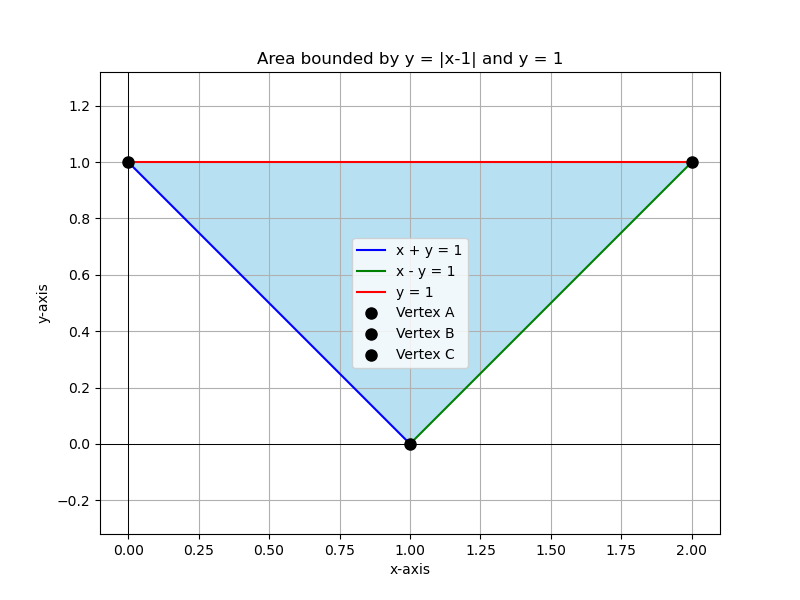
\includegraphics[width=0.7\columnwidth]{figs/Figure_1.png}
    \label{fig:placeholder}
    \caption{1}
\end{figure}
\end{frame}
\end{document}